% -*- LaTeX -*- %%%%%%%%%%%%%%%%%%%%%%%%%%%%%%%%%%%%%%%%%%%%%%%%%%%%%%
%
% Template for scribing COMP163 - Computational Geometry 
%
% Spring, 2004
%
%%%%%%%%%%%%%%%%%%%%%%%%%%%%%%%%%%%%%%%%%%%%%%%%%%%%%%%%%%%%%%%%%%%%%%
%**start of header 

\documentclass [12pt]{article}
\usepackage{epsfig}
\usepackage{enumitem}
\usepackage{amsmath}
\usepackage[color, leftbars]{changebar}

\usepackage{caption}
\usepackage{subcaption}


\setlength{\textwidth}{6.5in}
\setlength{\textheight}{9in}
\setlength{\oddsidemargin}{0in}
\setlength{\evensidemargin}{0in}
\setlength{\topmargin}{-0.5in}

\setlength{\parindent}{0pt}

\newtheorem{theorem}{Theorem}[section]
\newtheorem{definition}[theorem]{Definition}
\newtheorem{claim}[theorem]{Claim}
\newtheorem{lemma}[theorem]{Lemma}
\newtheorem{proof}[theorem]{Proof}

\newlength{\toppush}
\setlength{\toppush}{2\headheight}
\addtolength{\toppush}{\headsep}

\usepackage{hyperref}
\hypersetup{
    colorlinks=true,
    linkcolor=blue, % was previously black
    filecolor=magenta,
    urlcolor=blue,
    pdftitle={Template}
}
\urlstyle{same}

%\doheading{2}{title}{Last Revised: January, 2004}
%\htitle{title}

\def\subjnum{Comp 163}
\def\subjname{Computational Geometry}

\def\doheading#1#2#3{\vfill\eject\vspace*{-\toppush}%
  \vbox{\hbox to\textwidth{{\bf} \subjnum: \subjname \hfil Amy Bui}%
    \hbox to\textwidth{{\bf} Tufts University, Fall 2022 \hfil#3\strut}%
    \hrule}}

\newcommand{\htitle}[1]{\vspace*{3.25ex plus 1ex minus .2ex}%
\begin{center}
{\large\bf #1}
\end{center}} 

%%%%%%%%%%%%%%%%%%%%%%%%%%%%%%%%%%%%%%%%%%%%%%%%%%%%%%%%%%%%%%%%%%%

\begin{document}
% \doheading{2}{title}{Project} 
% \htitle{Line Segment Intersection Test Shots}
% \bigskip 
% \bigskip 
%%%%%%%%%% begin text after this line %%%%%%%%%%%%%%

\begin{figure}[h] %%%%%%%%%%%%%%%%%%%%%%%%%%%%%%%%%%%%%%%%
    \begin{tabular}{cc}
        \begin{subfigure}{0.5\textwidth}
            \centering
            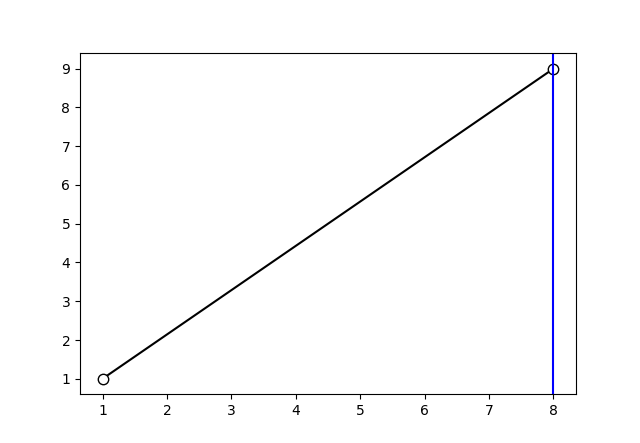
\includegraphics[width=\textwidth]{images/1Line.png}
            \caption{Base Case: 1 Predefined Line}
        \end{subfigure} &
        \begin{subfigure}{0.5\textwidth}
            \centering
        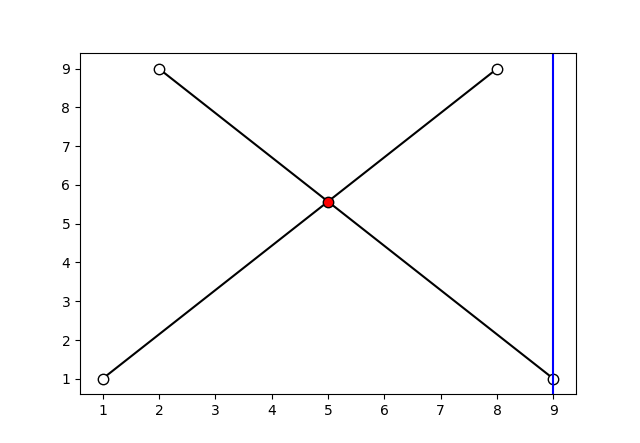
\includegraphics[width=\textwidth]{images/2Lines.png}
        \caption{Simple Case: 2 Predefined Lines}
        \end{subfigure} \\ 
        \begin{subfigure}{0.5\textwidth}
            \centering
            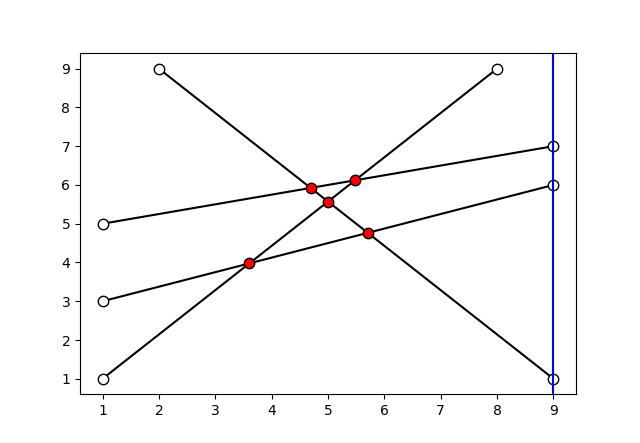
\includegraphics[width=\textwidth]{images/4Lines.png}
            \caption{Simple Case: 4 Predefined Lines}
        \end{subfigure} &
        \begin{subfigure}{0.5\textwidth}
            \centering
            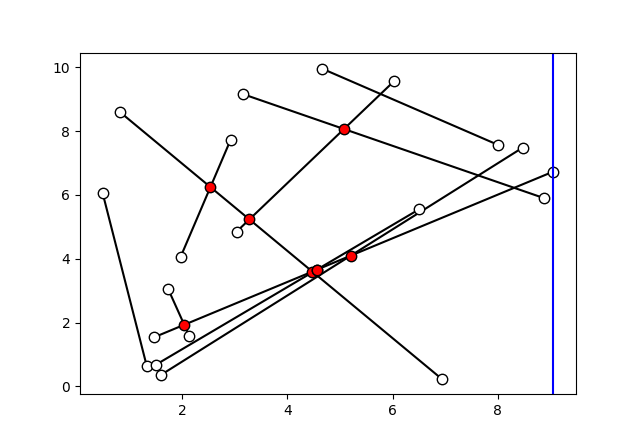
\includegraphics[width=\textwidth]{images/10LinesWrong.png}
            \caption{10 Random Lines, missing intersections}
        \end{subfigure} \\
        \begin{subfigure}{0.5\textwidth}
            \centering
        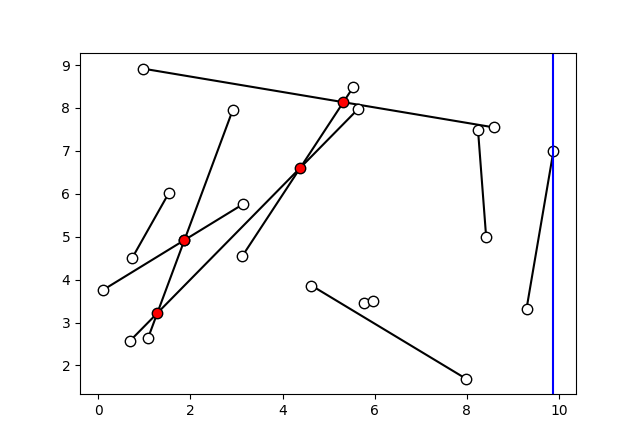
\includegraphics[width=\textwidth]{images/10LinesOkay.png}
        \caption{10 Random Lines, all results}
        \end{subfigure} &
        \begin{subfigure}{0.5\textwidth}
            \centering
        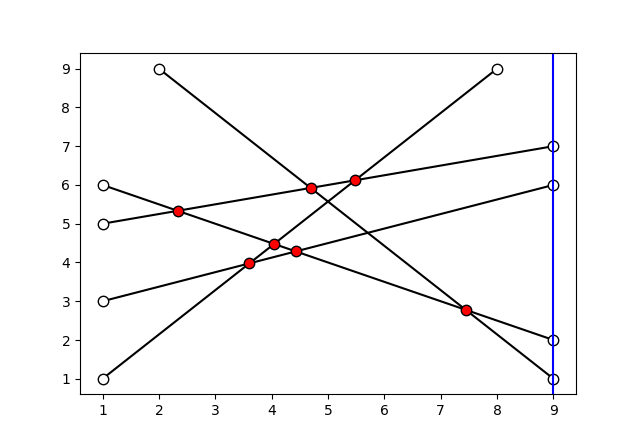
\includegraphics[width=\textwidth]{images/5LinesWrong.png}
        \caption{5 Predefined Lines, missing intersections}
        \end{subfigure}
    \end{tabular}
\end{figure}

% \begin{figure}[h]
%     \centering
%     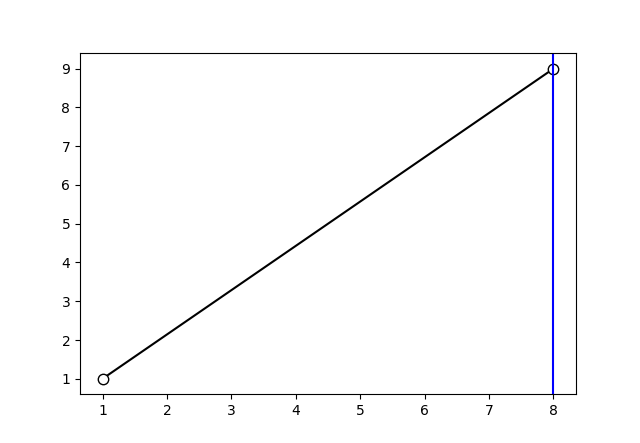
\includegraphics[width=0.5\textwidth]{images/1Line.png}
%     \caption{Base Case: 1 line}
% \end{figure}

% \begin{figure}[h]
%     \centering
%     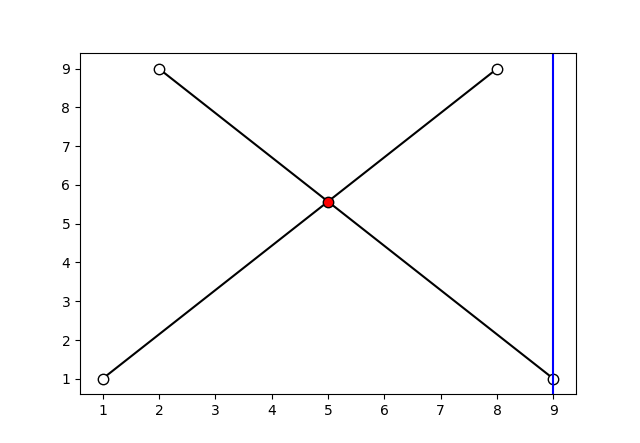
\includegraphics[width=0.5\textwidth]{images/2Lines.png}
%     \caption{Simple Case: 2 Lines}
% \end{figure}

% \begin{figure}[h]
%     \centering
%     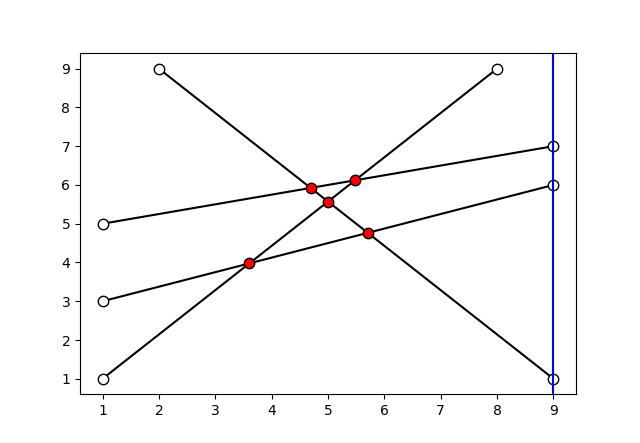
\includegraphics[width=0.5\textwidth]{images/4Lines.png}
%     \caption{Simple Case: 4 Lines}
% \end{figure}

% \begin{figure}[h]
%     \centering
%     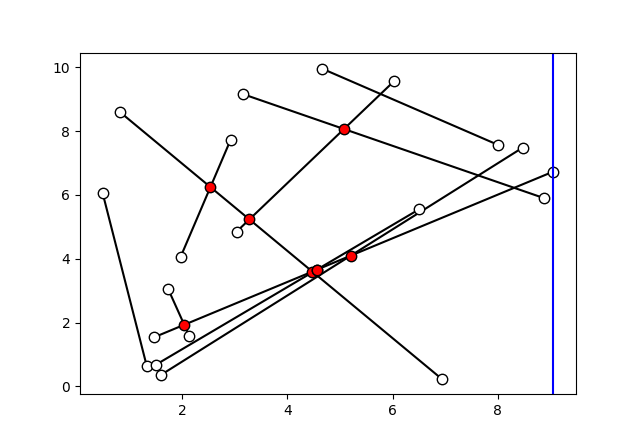
\includegraphics[width=0.7\textwidth]{images/10LinesWrong.png}
%     \caption{10 Lines, missing intersections}
% \end{figure}

% \begin{figure}[h]
%     \centering
%     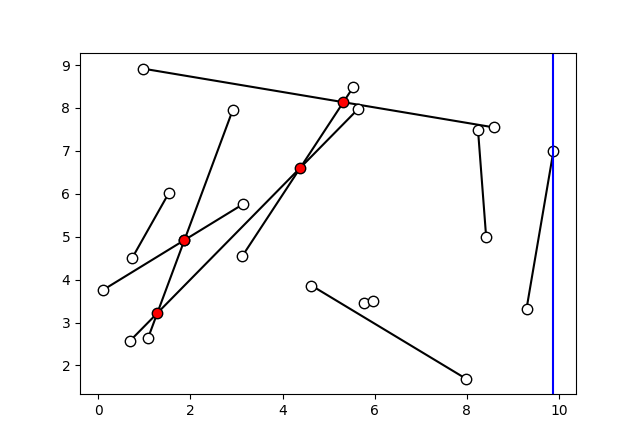
\includegraphics[width=0.7\textwidth]{images/10LinesOkay.png}
%     \caption{10 Lines, all results}
% \end{figure}

%%%%%%%%%%%%%%%%%%%%%%%%%%%%%%%%%%%%%%%%%%%%%%%%%%%%%%%%%%%%%%%%%%%%%%
\end{document}
%%%%%%%%%%%%%%%%%%%%%%%%%%%%%%%%%%%%%%%%%%%%%%%%%%%%%%%%%%%%%%%%%%%%%%

